\documentclass[11pt]{article}
\usepackage[T1]{fontenc}
\usepackage[utf8]{inputenc}
\usepackage[french]{babel}
\usepackage{array}
\usepackage[right=2.5cm, bottom=2.5cm,top=2.5cm, left=2.5cm]{geometry}
\usepackage{graphicx}
\usepackage{subfigure}
\DeclareGraphicsExtensions{.pdf,.eps,.jpg,.png,.gif}

\usepackage{color}


\usepackage[procnames]{listings}
\definecolor{codegreen}{rgb}{0,0.6,0}
\definecolor{codegray}{rgb}{0.5,0.5,0.5}
\definecolor{codepurple}{rgb}{0.58,0,0.82}
\definecolor{backcolour}{rgb}{0.95,0.95,0.92}
 
\lstset{language=Python, 
    backgroundcolor=\color{backcolour},   
    commentstyle=\color{codegreen},
    keywordstyle=\color{magenta},
    numberstyle=\tiny\color{codegray},
    stringstyle=\color{codepurple},
    basicstyle=\footnotesize,
    breakatwhitespace=false,         
    breaklines=true,                 
    captionpos=b,                    
    keepspaces=true,                 
    numbers=left,                    
    numbersep=5pt,                  
    showspaces=false,                
    showstringspaces=false,
    showtabs=false,                  
    tabsize=2
}

\title{\vspace{\fill} Cryptographie et sécurité \\ ~\textbf{IFT-606} \\~\\ Rapport de projet - La Brulerie}
\author{Amandine Fouillet - 14 130 638  ~\\ Frank Chassing - 14 153 710 ~\\ Thomas Signeux - 14 126 590}
\date{\today \vspace{\fill}}

\begin{document}
\maketitle
\newpage \thispagestyle{empty}
\null
\newpage
\tableofcontents
\newpage
\section*{Introduction \markboth{INTRODUCTION}{}}
\addcontentsline{toc}{section}{Introduction}

Avec la multiplication des objets connectés, notamment les smartphones et autres appareils mobiles, de nombreux réseaux publics ont vu le jour dans divers endroits. Cependant, la sécurité de ces réseaux est parfois douteuse et il est aisé de s’y introduire, à l'insu de tous. Une fois sur ces réseaux, les possibiltés d'intrusions et de malveillances sont nombreuses. Parmi ces intrusions, l'une d'elles peut être particulièrement efficace et dangereuse pour les personnes visées. Cette attaque se nomme Man In The Middle.

Ce projet a pour but d'étudier cette faiblesse du réseau en développant une application capable de reproduire les principales attaques Man In the Middle mais également de pouvoir s'en protéger.

\section{Description du projet et des objectifs}

\subsection{L'attaque Man In The Middle}
L’attaque Man In The Middle a pour but d’intercepter les communications transitant entre deux machines, sans que ni l’une ni l’autre ne se doute que le canal de communication est compromis.
L’attaquant a alors la possibilité de lire mais aussi de modifier les messages  (dans une certaine mesure).

Il existe plusieurs techniques pour se faire passer pour l'une ou l'autre de ces machines cibles.

\begin{itemize}
	\item l'ARP Spoofing : attaque la plus fréquente, utilisée dans la partie pratique de ce projet. On force les communications à transiter par l'ordinateur de l'attaquant qui se fait alors passer pour le routeur (gateway) du réseau.
	\item le DNS Poisoning : le but de cette attaque est de faire correspondre l'adresse IP d'une machine controlée par un pirate à un nom réel et valide d'une machine publique. Pour cela, il altère le ou les serveur(s) DNS du réseau.
	\item l'analyse du trafic : technique de sniffing permettant de visualiser les informations non chiffrées.
	\item le déni de service : empêcher le fonctionnement d'une machine pour en prendre le contrôle.
\end{itemize}


\subsection{Objectifs initiaux}
L’objectif de ce projet est de mettre en place des scénarios d’attaques de piratage de réseaux et de proposer des moyens de défense. Dans un premier temps, nous explorerons l'actualité des attaques de réseaux publics. Puis nous présenterons le travail réalisé lors du projet. Enfin, nous verrons les chapitres liés aux descriptions techniques du projet ainsi qu'un guide d'utilisation.~\\

Voici les principaux objectifs que nous nous sommes fixés avant de commencer le développement de notre application :

\begin{itemize}
\item Pouvoir identifier les ordinateurs connectés au routeur
\item Couper l’ensemble des connexions au routeur afin de bénéficier d’une meilleure bande passante
\item Limiter la connexion des personnes connectées au réseau
\item Récupérer les informations transitant sur les réseau pour pouvoir les analyser et identifier les personnes se trouvant dans le bar
\item Organiser une défense aux attaques précédentes
\item Faire une vidéo de présentation 
\end{itemize}

\section{Présentation du travail réalisé}
Afin de répondre à nos différents objectifs nous avons décidé de mettre en place plusieurs attaques contre des utilisateurs connectés sur le même réseau que nous. Pour faciliter le déroulement des attaques nous avons créé une interface graphique simple qui permet à l'attaquant de mener des offensives contre sa victime en quelques clics. De façon à proposer un outil polyvalent, nous avons également introduit dans l'interface une fenêtre de défense avec deux différents types de protection implémentés. ~\\

Pour réaliser les attaques, la défense et l'interface graphique nous avons utilisé un seul langage de programmation, le langage Python. Outre sa portabilité, ce langage offre une multitude de librairies déjà implémentées pour la manipulation de paquets réseau notamment le module Scapy que nous avons utilisé pour réaliser chacune de nos attaques et défenses. Ce module permet de forger, envoyer, réceptionner et manipuler des paquets réseau.~\\

Dans cette seconde section, nous allons présenter les scripts que nous avons implémentés, leur rôle et surtout leur fonctionnement.
\subsection{Attaque}
Nous avons implémenté trois différentes attaques : l'identification des utilisateurs sur le réseau, la coupure de ces usagers et enfin la récupération des liens internet qu'ils visitent. La première attaque est toujours effectuée car sans elle, il nous est impossible d'effectuer les suivantes. Par contre les attaques de coupure et d'écoute, même si elles se ressemblent, ont été implémentées séparément. Ci dessous, nous allons décrire les différentes attaques, leur réalisation et leur fonctionnement à travers l'interface graphique.
\subsubsection{Identification}
Cette attaque consiste à analyser le réseau auquel l'attaquant est connecté et donner la liste de tous les utilisateurs présents et actifs sur ce même réseau. Ces usagers sont représentés par leur adresse IP et leur adresse MAC et ces identifiants seront utilisés pour cibler une victime lors des attaques suivantes. ~\\

\textbf{Identifier le réseau automatiquement}~\\

Toujours dans l'optique de permettre à l'utilisateur de communiquer seulement à travers une interface graphique, nous avons souhaité mettre en place une identification automatique du réseau ainsi que de la plage d'adresse IP à scanner. Pour cela, nous avons eu recours à deux modules python : \textit{netifaces} et \textit{netaddr}. Grâce au premier, on peut parcourir la liste des interfaces de l'attaquant et récupérer celle qui est utilisée pour la connexion au réseau, puis on peut récupérer l'adresse IP locale de l'attaquant ainsi que le masque de sous-réseau. Puis, avec netaddr on effectue des opérations sur les adresses IP afin de trouver l'adresse et la plage d'adresse du réseau. ~\\
\lstinputlisting[caption=Identification du reseau]{./Codes/identifier1.py}~\\

\textbf{Envoi d'une requête ARP}~\\

Maintenant que l'on a identifié la plage d'adresse du réseau auquel l'attaquant est connecté, on va envoyé une requête ARP a chaque adresse de cette plage. Pour cela, on utilise la fonction \textit{srp} de scapy qui envoie et reçoit des paquets de la couche de liaison de données.~\\
\lstinputlisting[caption=Envoi d'une requête ARP]{./Codes/identifier2.py}~\\
\textbf{Récupération des ordinateurs connectés}~\\

Seuls les ordinateurs connectés vont répondre et nous pourrons ainsi récupérer leur adresse IP et leur adresse Mac. Il nous suffit de parcourir le résultat de la fonction srp et d'enregistrer dans une liste les ordinateurs qui ont répondu.~\\
\lstinputlisting[caption=Récupération des réponses]{./Codes/identifier3.py}~\\

\textbf{Lien avec l'interface}~\\

Au niveau de l'interface, l'identification se lance automatique à l'appui sur le bouton "Attaquer" de la page principale. Le script d'identification retourne à l'interface la liste des ordinateurs connectés et on les affiche sous forme d'une liste dans la fenêtre d'attaque. Il est également possible d'actualiser l'identification une fois sur la fenêtre d'attaque grâce au bouton "Actualiser", le script d'identification est relancé et la liste des machines connectées est mise à jour.

\subsubsection{Coupure}
Cette attaque consiste simplement a couper la connexion au réseau d'une autre machine. Pour la réaliser, on met en place l'attaque Man In The Middle en envoyant des faux paquets à la victime et à la gateway. Le module scapy permet de créer et d'envoyer ces faux paquets.~\\

\textbf{Création des faux paquets}~\\

On crée les deux faux paquets : le premier pour se faire passer pour la gateway auprès de la victime et le second pour se faire passer pour la victime auprès de la gateway.~\\
\lstinputlisting[caption=Création des faux paquets]{./Codes/couper1.py}

\textbf{Envoi des paquets}~\\

On envoie les deux paquets grâce à la fonction \textit{send} de scapy qui envoie des paquets sur la couche réseau.~\\
\lstinputlisting[caption=Envoi des paquets]{./Codes/couper2.py}
\newpage
\textbf{Sniff}~\\

Après un moment, la véritable gateway envoie un ARP, la victime n'est alors plus trompée car la communication ne passe plus par l'attaquant. Pour empêcher cela, on écoute la communication entre la gateway et la victime et dès que la gateway envoie une réponse ARP, l'attaquant usurpe la victime.~\\
\lstinputlisting[caption=Sniff de la communication victime gateway]{./Codes/couper3.py}

\textbf{Lien avec l'interface}~\\

Dans l'interface, la coupure peut se réaliser en sélectionnant une victime dans la liste des machines connectées au réseau et en appuyant sur le bouton couper. Pour chaque machine allant être coupée, le programme crée un thread qui appelle le script de coupure. Ainsi, il est possible de couper une ou plusieurs machines et continuer d'utiliser l'interface. ~\\
\lstinputlisting[caption=Lancement d'un thread de coupure]{./Codes/mainGraphique2.py}~\\

Lorsque l'attaquant souhaite rétablir la connexion de la victime, il peut appuyer sur le bouton rétablir, et le thread se termine.~\\
\lstinputlisting[caption=Arrêt d'un thread de coupure]{./Codes/mainGraphique3.py}

\subsubsection{Récupération des paquets}
Lors de cette attaque, on veut, en quelque sorte, espionner la victime en ayant accès à la liste de ses visites sur internet. Comme lors de l'attaque précédente, pour avoir accès aux données échangées entre la victime et la gateway, il faut réaliser une attaque Man In The Middle afin de se placer entre les deux et récupérer les paquets échangés.~\\

\textbf{Man In The Middle}~\\

On commence par mettre en place l'attaque Man In The Middle en envoyant des faux paquets ARP comme lors de l'attaque précédente. Mais, cette fois ci nous voulons que la victime conserve un accès à internet afin d'observer ses visites. On envoie donc les faux paquets toutes les 1,5 ms.~\\
\lstinputlisting[caption=Man in the middle]{./Codes/attaque.py}

\textbf{Ecoute}~\\

Pour observer la victime on lance une écoute sur son adresse IP. Etant donné que l'on se fait passer pour la gateway, la victime nous envoie directement ses paquets et nous pouvons les analyser grâce à la fonction http\_header.~\\
\lstinputlisting[caption=Traitement des paquets]{./Codes/ecoute1.py}

La fonction http\_header récupère tous les paquets et les analyse afin de récupérer les informations qui nous intéressent. Pour le cadre ce projet, nous nous sommes concentrés dans la récupération des adresses internet visitées. Pour retrouver cette adresse au milieu d'un paquet, on commence par repérer le champ GET afin d'être sûr que l'on a un paquet html. Ensuite, on récupère seulement les données en en-tête du paquets qui sont encapsulées dans le champ Raw.  Parmis ces données, on recherche le champ "Host" et on récupère les données qui se trouvent après ce champ. 
Une fois ces données récupérées, nous pouvons récupérer plusieurs informations : 
\begin{itemize}
\item L'adresse du serveur de la page web visitée par la victime, située juste après le champ "Host".
\item L'adresse exacte de la page web visitée par la victime, située juste après le champ "Referer".
\item Des informations sur l'OS de la victime et le navigateur utilisé, situées juste après le champ "User-Agent".
\end{itemize}
On ne trouve pas toujours toutes les données dans un paquet c'est pourquoi nous avons décidé de récupérer l'adresse du serveur si l'adresse exacte n'était pas présente. Pour effectuer cette récupération d'informations et les recherches dans les paquets nous avons utilisé des expressions régulières et le module \textit{regex} de Python.
 ~\\
\lstinputlisting[caption=Récupération des réponses]{./Codes/ecoute2.py}

\textbf{Lien avec l'interface}~\\

Pour effectuer une attaque d'écoute, l'utilisateur doit sélectionner sa victime dans la liste et cliquer sur le bouton sniffer. Ce bouton lance alors deux threads en parallèle. Le premier exécute le script de l'attaque et le second le script d'écoute.

\lstinputlisting[caption=Lancement des threads pour intercepter les paquets]{./Codes/mainGraphique1.py}

\subsection{Défense}
Dans cette section, nous allons présenter nos applications de défense.
Afin de contrer les attaques ciblées sur une machine, nous avons déployé deux scripts. Le premier réalise une détection pour savoir si la machine est victime d'une attaque ARP spoofing. Le second script est une simple commande qui permet de contrer la coupure de connexion. ~\\

\subsubsection{Détection}

La première parade pour se protéger d'une attaque de type Man In The Middle est de pouvoir la détecter. C'est ce que nous allons voir dans cette section. 

Du point de vue théorique, lorsque l'on effectue un ARP poisoning, on cherche à faire passer sa propre machine pour le routeur auprès des autres machines du réseau. Comme nous l'avons vu dans la mise en place de l'attaque, on remplace l'adresse MAC du routeur par l'adresse MAC de la machine pirate. Ce changement n'est pas visible directement mais est pourtant bien présent dans les informations contenues dans les paquets. ~\\
Ce sont ces informations que notre script de détection va intercepter. En pratique, la fonction \textit{packetfilter} va récupérer les informations suivantes: ~\\
\begin{itemize}
	\item L'adresse IP de la source
	\item L'adresse MAC de la source
	\item L'adresse IP de destination
	\item L'opération du paquet
\end{itemize} ~\\
\lstinputlisting[caption=Récupération des informations du paquet]{./Codes/packetfilter.py}~\\

Si les informations recueillies ne sont pas cohérentes, nous les vérifions grâce à la fonction \textit{checkspoof}. ~\\
\lstinputlisting[caption=Vérification de la cohérence des informations]{./Codes/checkspoof.py}~\\

Si la source du paquet concerné n'est pas clairement identifiée (présente dans la \textit{list requests}) et si l'adresse ne correspond pas, on suppose qu'une attaque est en cours. L'adresse MAC associée à l'adresse source est enregistrée dans un fichier.
Si la source était présente dans \textit{list requests}, on la supprime de cette liste et on continue le traitement.~\\
\lstinputlisting[caption=Traitement graphique]{./Codes/detection.py}~\\

Graphiquement, après avoir sélectionné Défense dans le menu de l'application, l'option Détection permet de lancer ce programme. C'est la fonction \textit{detection} qui s'en charge. Après traitement des données, on lit un fichier où est stocké le résultat de notre détection:
\begin{itemize}
	\item Si le fichier est vide, aucune attaque n'est détectée, on affiche le message "Vous n'êtes pas attaqué"
	\item Si le fichier n'est pas vide, il contient l'adresse MAC de la machine pirate. Un message d'alerte est alors affiché en précisant l'adresse pour permettre d'identifier l'auteur de l'attaque.
	
\end{itemize}



\subsubsection{Anti-coupure}
Lors de nos recherches, nous avons également trouvé un script complet permettant de se protéger des attaques de coupure de connexion. Nous n'avons malheureusement pas eu assez de temps pour implémenter notre propre solution mais nous avons décidé d'utiliser le script afin d'offrir tout de même cette défense dans notre application.

Ce code permet, via le choix d'option, de commencer ou d'arrêter la protection. ~\\
	\lstinputlisting[caption=Choix des options]{./Codes/startstopanti.py}~\\
	
Graphiquement, c'est cet appel de fonction qui est utilisé pour lancer ou arrêter la protection. La protection est activable dans l'interface grâce à l'utilisation du bouton Anti-Coupure.~\\
	\lstinputlisting[caption=Code Anti-coupure]{./Codes/anticoupure.py}~\\	
	
	Dans le code, après définition des différentes fonctions appelées, on retrouve la partie à proprement utilisée. elle se situe dans la fonction \textit{startAntinetcut}	
	Dans cette fonction, on définit notre adresse IP et MAC. L'information est automatiquement récupérée.~\\
		\lstinputlisting[caption=Récupération des informations]{./Codes/IPMAC.py}~\\
		
		Puis, notre défense va se mettre en place. Pour cela, on va créer deux paquets, \textit{p1} et \textit{p2}: ~\\
		\lstinputlisting[caption=Créations des paquets]{./Codes/paquets.py}~\\
		Ces paquets permettent d'envoyer des requêtes ARP avec pour informations nos adresses MAC et IP à toutes les machines du réseau.
		
		Enfin, une boucle va envoyer nos deux paquets. On utilise pour cela la fonction \textit{sendp()} qui permet d'envoyer des paquets en couche liaison de données du modèle OSI.
		Tant que le programme est activé, on envoie contiuellement nos paquets.~\\
		\lstinputlisting[caption=Boucle principale]{./Codes/boucle.py}~\\	


\section{Guide utilisateur}
\subsection{Interface principale}
Pour lancer l'application, il faut taper la ligne de commande : \textit{sudo python mainGraphique.py} sur un terminal en ayant pris soin de se placer dans le bon répertoire. Au lancement de l'application, une fenêtre principale apparaît avec un menu et deux boutons : Attaque et Défense. Par le biais du menu, vous pouvez quitter l'application ou bien consulter les auteurs de celle-ci. Le bouton d'attaque amène vers une autre fenêtre permettant d'effectuer des attaques sur des machines connectés au même réseau que vous. Quant au bouton Défense, il permet d'ouvrir une fenêtre dévoilant des fonctionnalités qui peuvent vous protéger contre notre application.
\begin{figure}[!h]
\centering
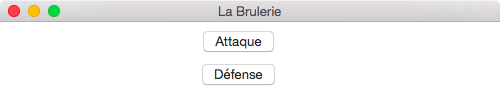
\includegraphics[scale=0.6]{./Captures/fenetrePrinc.png}
\caption{Fenêtre principale}
\end{figure}
\subsection{Attaque}
En cliquant sur le bouton Attaque, un scan du réseau s'effectue en un certain laps de temps et une nouvelle fenêtre s'ouvre avec une liste des ordinateurs connectés au même réseau. On retrouve des informations telles que l'adresse IP et l'adresse Mac des machines. En dessous de cette liste, vous trouverez quatre boutons  correspondant chacun à une fonctionnalité différente. Sous ces quatre boutons, on retrouve une seconde liste vide qui sera destinée à afficher les machines ayant la connexion coupée.
\begin{figure}[!h]
\centering
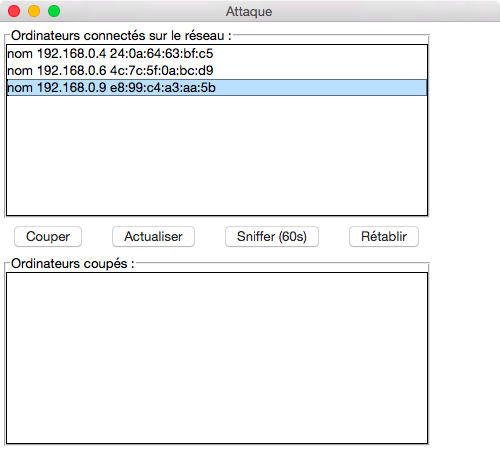
\includegraphics[scale=0.5]{./Captures/identificationFen.png}
\caption{Liste des machines connectées sur le réseau}
\end{figure}
\subsubsection{Couper et rétablir}
Afin de couper la connexion d'un ordinateur présent sur le réseau, vous devez sélectionner dans la liste des machines celles que vous voulez couper. Lorsque vous avez effectué la sélection, il suffit de cliquer sur le bouton Couper afin de couper la connexion des ordinateurs sélectionnés. Vous devriez ainsi apercevoir les machines coupées dans la seconde liste.~\\
Pour rétablir leur connexion il suffit de sélectionner les machines dont on veut rétablir la connexion dans la seconde liste, puis de cliquer sur le bouton Rétablir. Cela replacera les machines dans la première liste.
\begin{figure}[!h]
\centering
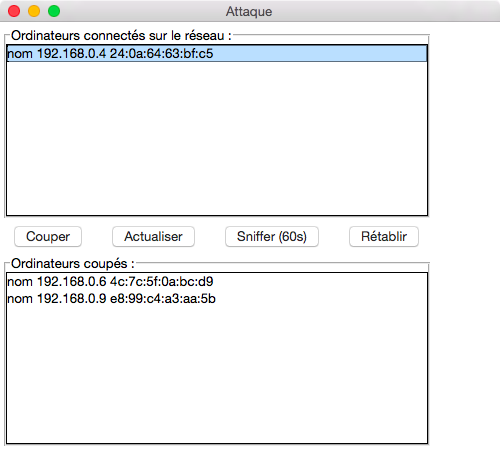
\includegraphics[scale=0.5]{./Captures/couperFen.png}
\caption{Coupure d'un ordinateur}
\end{figure}
\newpage
\subsubsection{Sniffer}
Pour procéder à une écoute réseau d'une machine, il suffit de sélectionner la machine que l'on veut écouter dans la première liste puis de cliquer sur le bouton Sniffer. Il faut alors attendre plusieurs secondes le temps d'écouter, puis une nouvelle fenêtre s'ouvre où l'on retrouve dans une liste les différents sites web que la machine a consulté ainsi que les différents serveurs par lequel elle est passée. Si rien n'a été capturé, un message explicite apparaît dans la liste pour avertir que rien n'a été capturé.
\begin{figure}[!h]
\centering
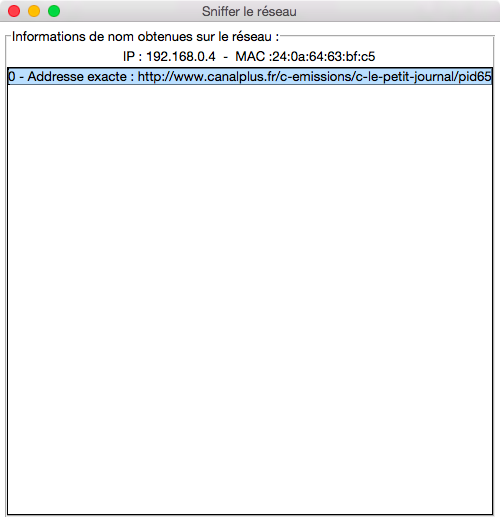
\includegraphics[scale=0.5]{./Captures/sniffFen.png}
\caption{Capture des paquets d'une victime}
\end{figure}

\subsubsection{Actualiser}
Sur la fenêtre d'attaque, le bouton Actualiser permet d'actualiser la liste des ordinateurs connectés au réseau. Cela prend quelques secondes pour effectuer le scan de nouveau. Pour exécuter cette action, il faut qu'aucune machine ne soit coupée.

\newpage
\subsection{Défense}
La fenêtre de défense se compose de seulement deux boutons : Le bouton de détection d'une attaque et le bouton d'anti-coupure.
\begin{figure}[!h]
\centering
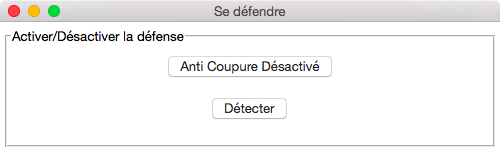
\includegraphics[scale=0.6]{./Captures/defense.png}
\caption{Fenêtre de défense}
\end{figure}

\subsubsection{Détecter une attaque}
Si l'on clique sur le bouton de détection d'une attaque, cela va vérifier tout simplement si vous êtes en train de vous faire attaquer. Au bout de quelques secondes, une boite de dialogue s'ouvre et vous affiche si oui ou non vous êtes attaqués. Dans le cas où vous êtes attaqués, vous aurez l'adresse Mac de la machine attaquante.
\begin{figure}[!h]
\centering
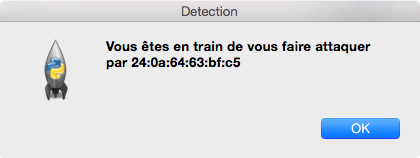
\includegraphics[scale=0.6]{./Captures/detection.png}
\caption{Pop-up de détection d'attaque}
\end{figure}
\subsubsection{Activer une protection contre les coupures}
Si l'on active le bouton de protection contre les coupures, votre connexion internet ne pourra plus être coupée. Vous pourrez ainsi naviguer sans inquiétude sur Internet.




\section{Planification et organisation}
Dans cette section, nous allons décrire comment nous avons organisé le développement de l'application et quels outils nous avons utilisés.

\subsection{Outils utilisés}
Ce projet a nécessité l'utilisation d'un certain nombre d'outils qui sont détaillés dans le tableau ci-dessous.~\\
\begin{figure}[h]
\centering
\begin{tabular}{|l|l|}
\hline
   \textbf{Python} & Langage utilisé pour sa polyvalence et son efficacité dans le développement de  \\
    &code pour la sécurité. \\ \hline
    \textbf{Scapy} & Framework basé sur Python fournissant un grand nombres de fonctions pour  \\
    & manipuler les paquets réseau. \\ \hline
   \textbf{Google Drive} & Le début du développement s'est fait grâce à la plateforme de création et  \\
	& de partage de fichiers de Google. \\ \hline
\textbf{Github} & Site d'hébergement et de gestion pour le développement informatique. Nous \\ 
&   l'avons utilisé pour partager le code et les notes afin que chacun puisse suivre   \\
&  le travail des autres. \\ \hline
\textbf{iMovie} & Logiciel qui nous a permis de réaliser le montage des vidéos de présentation \\ \hline
\textbf{LaTeX} & Les fonctonnalités du langage LaTeX ont permis la rédaction du rapport final. \\ \hline
\textbf{Prezi} & Logiciel de présentation intéractif, utilisé pour la confection de la présentation \\
& finale.\\ \hline
\end{tabular}
\caption{Outils utilisés}
\end{figure}

\subsection{Planification}
Ce projet nécessitait une certaine organisation au niveau de la réalisation des tâches. C'est pourquoi nous avons déterminé une logique de planification s'étendant sur 5 semaines nous permettant ainsi de pouvoir atteindre nos objectifs en respectant les délais. De plus, le suivi hebdomadaire avec Mr Ouenzar nous a aidé à remédier à nos difficultés qui pouvaient nous freiner dans le développement de l'application. ~\\
Ci-dessous un tableau récapitulatif des différentes tâches que nous avions prévues de réaliser par semaine et les différentes tâches que nous avons finalement réalisé durant ces semaines.~\\

\begin{figure}[h]
\centering
\begin{tabular}{|l|l|l|l|}
\hline
Sem. & Tâches prévues & Tâches réalisées &Temps\\ \hline

1& Détermination du sujet  &Détermination du sujet& 6h/pers \\
& Recherches/Documentation &Recherches/Documentation& \\
& Elaboration des objectifs &Elaboration des objectifs &  ~\\ \hline

2& Développement de l'identification  &  Identification &8h/pers \\
& Mise en place de l'interface graphique & Mise en place de l'interface graphique& \\
&  Développement de la détection & Recherches& ~\\ \hline

3& Développement de la coupure &Développement de la coupure& 10h/pers \\
& Identification dans l'interface &Identification dans l'interface& \\
&Développement de l'anti-coupure&Développement de la détection & ~\\ \hline

4& Développement de l'écoute &Développement de l'écoute& 10h/pers \\
& Tests des modules réalisés& Intégration coupure, détection et écoute&\\
& Intégration de la coupure et détection&& ~\\ \hline

5& Tests des modules réalisés&Tests des modules réalisés &16h/pers \\
& Réalisation de la vidéo & Intégration du script anti-coupure&\\
& Réalisation du Prezi &Prezi &\\
& Rédaction du rapport &Rapport& \\
& &Vidéo&  \\ \hline
\end{tabular}
\caption{Planification}
\end{figure}

\subsection{Répartition des tâches}
Afin de tester notre application nous avions besoin d'un routeur sur lequel on puisse effectuer nos attaques. Nous avions à notre disposition qu'un seul routeur qui nous permettait de faire les tests, c'est pourquoi nous nous réunissions toujours le lundi afin de travailler et tester nos réalisations.
Nous nous sommes répartis le travail de la façon suivante :  
\begin{itemize}
	\item Amandine s'occupe de la partie attaque (identification, coupure, écoute) du projet
	\item Frank est en charge de la partie graphique et de l'intégration des différents modules
	\item Thomas développe les modules de défense (détection et anti-coupure)
\end{itemize}
Notre cadre de travail nous permettait d'être chacun au courant de l'avancée du travail des autres. De plus, chaque membre du groupe expliquait ses réalisations aux autres membres du groupe afin que tout le monde puisse comprendre le projet dans sa globalité.
Nous avons effectué des tests le plus souvent possible, dès qu'un module était réalisé et dès que l'intégration graphique de ce module était réalisée. La réalisation de la vidéo nous a permis de faire un test de l'ensemble de l'application.
Après avoir défini ensemble le plan et la base du rapport, chaque membre du groupe en a rédigé la partie le concernant. Nous avons procédé de la même façon pour la réalisation des diaporamas.


\section{Améliorations et problèmes rencontrés}
\subsection{Perspectives}
Faute de temps, nous n'avons pas pu implémenter toutes les fonctionnalités que nous aurions voulu faire. Nous aurions aimé par exemple identifier le nom des machines connectées sur le réseau dès le scan du réseau, ce qui reste un élément important pour identifier une personne dans la même pièce que nous. Cependant, nous n'avons pas eu le temps de trouver un moyen de faire cela efficacement. Nous arrivons seulement à récupérer l'OS et le type de navigateur d'une machine mais nous ne l'avons pas ajouté à l'interface.~\\

Second point que nous aurions pu améliorer, c'est le fait de rajouter le code du ralentissement de connexion à l'interface graphique. En effet, ayant trouvé comment coder cette fonctionnalité vers la fin du projet, nous n'avons pas pu l'implémenter sur l'application.~\\

Egalement, au niveau de l'attaque, nous pourrions essayer d'obtenir plus d'informations sur les sites que visite la victime telles que son mail, son nom ou prénom, ses identifiants, etc. Nous aimerions aussi implémenter une fonction de sniff fonctionnant avec les sites https.~\\

Pour la défense, il se trouve qu'on hésitait à effectuer une détection en continu q'une attaque au lieu de détecter à un instant donné. Puis nous pourrions éventuellement récupérer plus d'informations sur l'attaquant. En ce qui concerne l'anti-coupure, ce script ne nous appartenant pas, nous n'avons pas réussi à faire en sorte qu'il s'arrête après son activation.~\\

D'autres fonctionnalités telles que le crack de clé WEP et WPA que nous avons vu durant nos devoirs pourrait venir se greffer à notre application. Toutes ces améliorations permettraient avant tout de rendre l'application plus complète et fiable.

\subsection{Problèmes rencontrés}
Lors du développement de notre application, nous nous sommes confrontés à plusieurs complications. Tout d'abord, nous utilisions tous les trois des systèmes d'exploitation différents ce qui posait quelques difficultés dans les phases de tests. Les tests ne pouvaient pas être effectués à partir d'une machine virtuelle. De plus, l'installation de certaines bibliothèques Python notamment Scapy était difficilement envisageable sur Windows car son installation est très compliquée.~\\

Fort heureusement, nous possédions une machine sur Mac OS et une machine sur Linux. Nous pouvions donc effectuer des phases de tests mais nous devions également faire en sorte que notre application fonctionne pour les deux OS.~\\

De plus, nous sommes plus ou moins novices dans la programmation Python et dans les librairies auxiliaires que le langage possède. Nous avons donc dû nous adapter et apprendre au fur et à mesure de nos besoins.

\section*{Conclusion \markboth{CONCLUSION}{}}
\addcontentsline{toc}{section}{Conclusion}
Nous avons finalement réussi à développer une application répondant à nos objectifs principaux. Nous pouvons ainsi, par le biais de celle-ci, obtenir l'ensemble des ordinateurs connectés à un réseau et effectuer des attaques de coupure de connexion ou bien d'écoute du réseau. Nous avons également la possibilité de se défendre contre notre propre application. Ce projet nous a avant tout permis de découvrir les faiblesses au niveau de la sécurité du réseau et d'implémenter des attaques de type Man In The Middle afin d'exploiter ces faiblesses. Il nous a notamment permis de consolider notre connaissance du langage Python et notre faculté à travailler en groupe. Cette expérience enrichissante nous a familiarisé à de nouveau outils de développement mais nous a aussi sensibilisé à la sécurité des réseaux.~\\

\begin{center}
Adresse de la présentation : \textbf{https://prezi.com/fgbay3xusqaw/}
\end{center}
\newpage
\listoffigures
\lstlistoflistings
\end{document}
